\subsubsubsection{Interlayer service}

This component is responsible of the communication that is performed between
different layers, namely the one which it belongs (the \textbf{middleware}) and
another one who uses the middleware layer, that is the \textbf{application}
layer.

We show in Figure \ref{fig:mw-interlayer} the architecture of this service and
then we will show in detail each module that composes this component.

\begin{figure}[H]
  \centering
  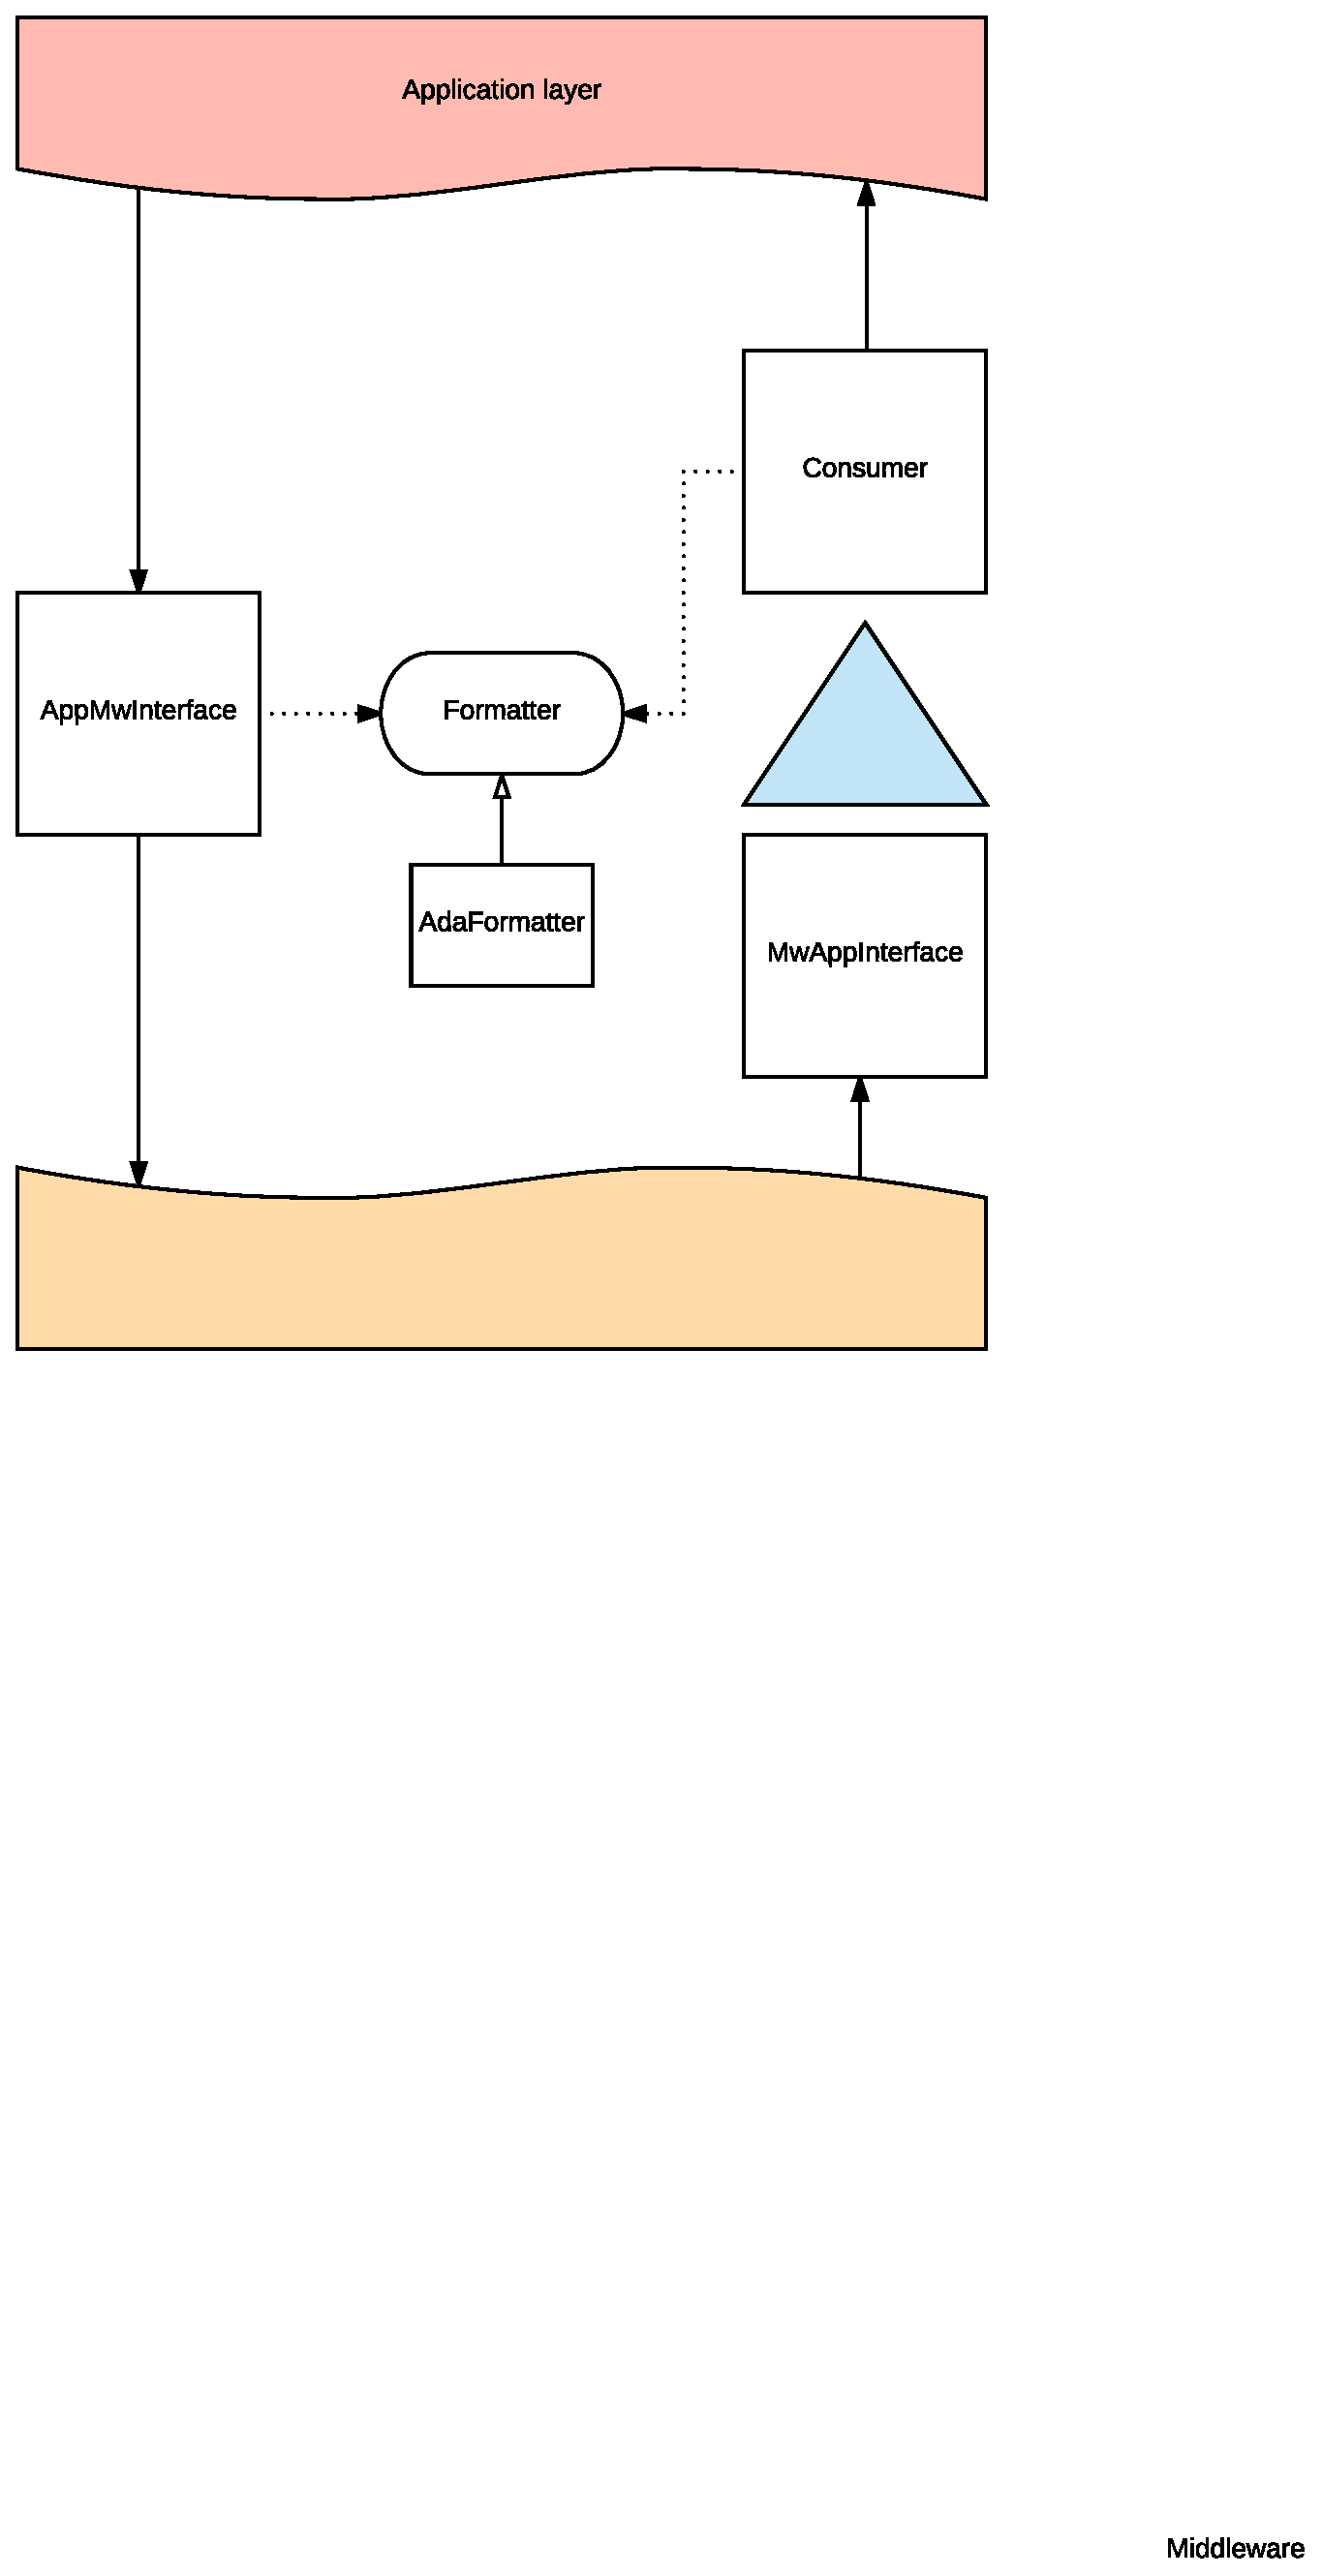
\includegraphics[width=.8\columnwidth]{images/solution/mw/int/architect.eps}
  \caption{Middleware's Interlayer service}
  \label{fig:mw-interlayer}
\end{figure}

We can see that the Interlayer service embodies two flows of information, each
one directed in the opposite direction as the other (the orange band represents
the middleware).

The \texttt{AppMwInterface} module just listens on a port waiting for messages
from the application layer and passes them to other services in the middleware.
It is capable of receiving different messages in parallel.

\texttt{MwAppInterface} receives requests by other middleware services to send
messages to the application layer. Instead of blocking the requesting process
on the delivery of the message, the latter gets stored in a Redis queue and
asynchronously handed over to the \texttt{Consumer} module by means of the
GenStage behaviour. When they demand work, \texttt{Consumer} instances send
pending messages to the application layer and, for each successful delivery,
pop the delivered message from the Redis queue.

Also, \texttt{Consumer}s can store meta-information for messages delivered to
the application. They do so in order to keep track of the RPCs performed by the
application layer, namely storing the logical name of the node which issued a
request in a Redis map. Then, when an RPC gets satisfied from the
application layer, \texttt{AppMwInterface} will correlate the answer with the
node which initially issued the request, and will forward the RPC result to it.
In fact, this feature allows us to preserve the transparency offered by the
middleware in the case of application-level RPCs.

Since some runtimes may handle strings in a different format with respect to
what Elixir does, we defined a \texttt{Formatter} behaviour for cope with these
issues.
We implemented a couple of formatters, one for Elixir (it does nothing but
return the message as it is) and one for Ada. In particular, Ada does not
output the actual character sequence when using \texttt{'Output}: in this case
the receiving sockets reads additional meta-information along with the string,
which are basically the boundaries of the binary data streamed.
However, this is not enough: in fact, we also had to split long messages since
Ada's Stream \texttt{'Input} attribute reads up to about 200B; therefore, the
\texttt{Consumer} module also has to split long messages into chunks in order
to deliver them without causing a failure during the reception.
